% Here is a suggested template for PhD research proposal for the
% first annual report.
% Written originally 2010-06-22 by T. W. Yee.
% Last modified      2018-06-15 by T. W. Yee.
% Last modified      2018-08-04 by T. W. Yee, incorporating
%                    sample-research-proposal-2.pdf from UoA.


\documentclass[12pt,a4paper]{article}


 \usepackage{natbib}    % For BibTeX
 \usepackage{graphicx}  % To import .pdf files
%\usepackage{times}
 \usepackage{float}
 \usepackage{amsfonts}
 \usepackage{amsmath}
 \usepackage{amssymb}
 \usepackage{listings}

 \oddsidemargin  -10mm
 \evensidemargin -10mm
 \headheight 0mm
 \headsep -3mm
\textheight 250mm
\textwidth 180mm
\topmargin -4mm
\topskip -10mm

%\textwidth=450pt
%\hoffset=-2cm


\newcommand{\RR}{{\textsf{R}}}


\begin{document}

\begin{Large}
\begin{center}
\textbf{``Principled and Efficient Interactive Data Visualization''} \\
\textbf{by Bartonicek, Adam} \\
\textbf{for a PhD in Statistics}
\end{center}
\end{Large}


\hfill{Student ID: 828803059}

\hfill{Email: abar435@aucklanduni.ac.nz}

\hfill{Department of Statistics}

Supervisor: Dr.~Simon~Urbanek
Co-supervisor: Dr.~Paul~Murrell


\begin{center}
Date of enrolment in the programme and expected date of completion
\end{center}

\begin{center}
February 1 2022, August 1 2025
\end{center}



This document represents the student's research proposal after
one year of provisional PhD registration.
Confirmed PhD registration is now sought.


% ----------------------------------------------------------------------
\section{Introduction}
\label{sec:intro}



Humans learn about the world around them by interacting with it. Further, as major part of our cerebral cortex is devoted to visual processing, we learn best by interacting with things that we can see. The same applies to data. If we want to learn from our data effectively, we need effective tools for visualizing data and interacting with it. As such, interactive data visualization is an important topic in statistics and data science. This is evidenced by the rising popularity of interactive visualization. Currently, many interactive data visualization libraries exists across popular data-science-adjacent programming languages (such R, Python, Julia, and Javascript) and their ecosystems, including D3 \citep{bostock2011}, plotly \citep{plotly2023}, Highcharts \citep{highcharts2023}, and Vega \citep{satyanarayan2015} and Vega-lite \citep{satyanarayan2016}. Yet, many of these present-day interactive data visualization libraries libraries suffer from a common set of drawbacks. Specifically, due to historical and other reasons (see Section \ref{sec:briefhistory} and \ref{sec:webinteractivity}), the libraries tend to fall into two categories: 

\begin{enumerate}

\item Specialized, high-level suites of "off-the-shelf" interactive visualizations.
\item Generic, highly customizable low-level frameworks.

\end{enumerate}

The libraries from the first camp are usually more approachable to users with less programming experience. This makes them very useful to specialists and applied researchers. However, a major drawback of these libraries is that they are not extendable - users cannot easily create new types of interactive plots, without delving into low-level implementation. As for the libraries from the second camp, these tend to lend the user a great deal of power and flexibility, however, to use them effectively, the users are required to have significant programming experience and deep knowledge of the specific library. This is especially true when it comes to implementing up complex interaction between multiple plots. Further, the responsibility for making sure that the interaction is coherent is left to the user: there is nothing stopping them from implementing interactive features that are meaningless, confusing, or unpredictable. Finally, the design philosophy behind many of these libraries seems to be oriented towards data presentation rather than data exploration \citep{batch2017}. As such, there is currently a lack of a \textbf{mid-level system} - one that would enforce a set of rules that would ensure the interaction is coherent while at the same time giving users the freedom to create a wide range of interactive figures - geared towards multiplot interaction and exploratory data analysis (EDA). 

The abovementioned absence of a mid-level is not just an implementation gap. Rather, it seems to be a symptom of an underlying lack of a strong theoretical foundation. Specifically, while many different types of interactive plots can be created and composed toghether, only some of these plot types and compositions will produce coherent graphics (see Section \ref{sec:coherency}). At the present time, there is no formal framework for determining ahead of time whether an interactive graphic will be coherent or not. As a consequence, the two options left to the creators of interactive data visualizations systems are either:

\begin{enumerate}

\item  Give the user a limited number of ready-made solutions that are known to behave well.
\item Put the onus of making sure that the interaction is coherent onto the user.

\end{enumerate}

These two options precisely map onto the two categories of extant interactive data visualization libraries outlined above. The goal of the proposed project is to find a third option and lay down the theoretical foundations for a mid-level interactive data exploration system, as well as implement it within a modern programming language. Specifically, at the theoretical level, I plan to map out the boundaries and constraints that parts of such an interactive data visualization system (e.g. datastructures and graphical primitives) need to satisfy in order to allow for coherent interactions. To this end, I will use concepts from category theory, an area of mathematics concerned with structure and composition (see Section \ref{ref:categorytheory}). At the applied level, I will implement the system in \textbf{JavaScript} and provide a high-level interface in \textbf{R}.  

% ----------------------------------------------------------------------
\section{Background}
\label{sec:background}

\subsection{What Event Counts as \textit{Interactive} Data Visualization?}
\label{sec:whatcounts}

It may seem surprising, but despite the widespread popularity of interactive data visualizations, there seems to be little consensus as to what actually makes a data visualization interactive. The term gets used by different researchers in vastly different contexts, sometimes in arguably conflicting ways. As such, for the purposes of the present text, it is important to disambiguate what is meant by "interactive data visualization".

Firstly, there is the issue of whether "interactive data visualization" refers to an object or system, or to an action, undertaken by a human being. \cite{pike2009} note that "interaction" is an overloaded term that can refer to either the concrete tools which users use to manipulate visual information or to the more abstract "human interaction with information" - the back-and-forth between the user and the visual information presented to them \citep[see also][]{yi2007}. The more abstract action definition is more often emphasized in the field of Human Computer Interaction \citep[see e.g.][]{sinha2010}. For the purpose of this text, the object/system definition will be used: interactive data visualizations are concrete objects that are produced by (typically computer-based) systems that take in data and produce visual images that can be interpreted and manipulated by humans \citep{brodbeck2009}.

\subsubsection{Simple Interactivity}

But even after narrowing down the focus to interactive data visualizations as objects, a lot of conceptual ambiguity remains. Some researchers use a \textbf{simple} definition and define interactive visualizations as any visualizations that can be actively manipulated by the user \citep{brodbeck2009}. Other researchers emphasize time or the \textbf{temporal} aspect, with visualizations being "interactive" when there is little lag between the user's input and changes to the visualization \citep{becker1987,buja1996}. Complicating the matters futher, some even make the distinction between "interactive" and "dynamic" manipulation, where interactive manipulation happens discretely, such as when pressing a button or selecting an item from a drop-down menu, whereas dynamic manipulation happens continuously, for example when smoothly moving a slider or by clicking-and-dragging \citep{rheingans2002,jankun2007model}. These tentative definitions present relatively little restriction on what counts as interactive visualization: for example, one could argue that the process of a user typing code into a command line to generate new plots could be considered interactive visualization, as long as it happens fast enough. 

\subsubsection{Complex Interactivity}

Other researchers do not seem to be satisfied with these broad definitions. For many, the defining feature of interactive data visualization is the ability to \textbf{query} different parts of the dataset (by e.g. zooming, panning, and filtering), and the reactive propagation of changes between connected or \textbf{"linked"} parts of interactive figures \citep{kehrer2012,buja1996,keim2002,unwin1999}. Similarly, in Visual Analytics (VA) research, a distinction is made between "surface-level" (or "low-level") interactions, which manipulate attributes of the visual domain only (e.g. zooming and panning), and \textbf{"parametric"} (or "high-level") interactions, which manipulate attributes of mathematical models or algorithms underlying the visualization \citep{leman2013,pike2009}. 

There are other ways that the term "interactive data visualization" has been used \citep[for more detailed taxonomies, see][]{yi2007}, however, short summaries of the key definitions mentioned above are presented in Table \ref{tab:definitions} and will be referred to later on in the text. What is important is that the different types of interactivity imply very different levels of programming complexity. For example, simply changing the color of a point or a bar in a plot, irrespective of anything else, might be implemented by changing an attribute of the underlying graphical primitive only - the point/bar does not need to know about what data it represents. However, if the change happens in response to (linked) brushing within a different plot, then there does need to be some way of tracking which cases of the data belong to the primitive. Likewise, changing the width of a histogram bar does not affect the graphical attributes of the bar only, but the underlying operation (binning) needs to be recomputed with respect to the new value of the parameter.  

\begin{table}[ht]
\caption{
Definitions of Interactive Data Visualization
}
\centering
\ ~~~~ \\
\label{tab:definitions}
\begin{tabular}{|p{2cm}|p{6cm}|p{8cm}|}
\hline
Name & Short Definition & Details \\
\hline

Simple & Change happens & User can manipulate the visualization in some way \\

Temporal & Change happens in real time & There is little lag between the user's input and changes to the visualization  \\

Querying & Change results from subsetting & The user can query different parts of the dataset, interaction is analogous to subsetting rows of the data (e.g. zooming, panning, and filtering) \\ 

Linked & Change propagates & Parts of the visualization are connected or “linked”, such that interaction with one part produces a change in another (e.g. linked brushing) \\

Parametric & Change reflects an underlying model & The user can manipulate the parameters of some underlying model (e.g. rotating principal axes in a PCA scatterplot, changing the width of a histogram bar) \\

(Cognitive) & Change is caused and perceived by a human & The user engages in a back-and-forth with the visual information presented to them \\

\hline
\end{tabular}
\end{table}

The conceptual ambiguity about what gets called "interactive" visualization matters because it leads to radically different implementations in software packages (see Sections \ref{sec:briefhistory} and \ref{sec:currentage}). For example, the \textbf{R Graph Gallery} page on \textbf{Interactive Charts} \citep{holtz2022} features several examples of interactive visualizations, however, none of them meet the linked and parametric definitions of interactivity outlined in Table \ref{tab:definitions}. Interactive data visualization systems that exist within the open source data visualization ecosystem differ significantly in the amount of features and flexibility they offer, as well as in how much responsibility or "house-keeping" for maintaining the interactive state they offload onto the user.     

\subsection{Brief History of Interactive Data Visualization in Statistics}
\label{sec:briefhistory}

\subsubsection{Static Visualization Goes Digital}

Static data visualization has a rich and intricate history \citep[see e.g.][]{dix1998,chen2008, friendly2021,young2011}. Briefly, for a long time, it was considered at best an auxiliary field, however, at the end of 1950's, a series of developments lead to a great increase in its prominence. Firstly, at the theoretical level, the work of Tukey (\citeyear{tukey1962,tukey1977}) and \cite{bertin1967} established data visualization as valuable discipline in its own right. Secondly, at the applied level, the development of personal computers \citep[see e.g.][]{abbate1999} and high-level programming languages, most notably FORTRAN in 1954 \citep{backus1978}, made production of figures easy and accessible to the wider public. Combined, these developments lead to a surge in the use and dissemination of data visualizations.

Final development in the field of static data visualization that is important to mention was the Grammar of Graphics introduced by Leland \cite{wilkinson2012}. Prior to Wilkinson's work, data visualization systems tended to come in two flavors: low-level ones, in which the users had to create visualizations from scratch using graphical primitives, and high-level ones, in which the users could select from a limited range of ready-made visualization types. Wilkinson, building upon the work of Bertin and Tukey, developed theory for a mid-level visualization system - Grammar of Graphics - which allows the users to specify a broad range of statistical graphics by declaratively combining abstract plot attributes such as aesthetics, scales, coordinates, and geometric objects \citep{wilkinson2012}. Grammar of Graphics has been successfully implemented in several software packages, most notably the popular \textbf{ggplot2} R package \citep{wickham2010} and the proprietary software \textbf{Tableau} \citep{tableau2023}. 

\subsubsection{Birth of Interactive Visualization}

As static visualization entered the computer age, interactive data visualization would not be left far behind. Early systems appeared in the 1960's and 1970's, and tended to be specialized for one specific task. For example, \cite{fowlkes1969} used interactive visualization to show how probability densities reacted to change of parameters and transformations, and \cite{kruskal1964} used interactive visualization to showcase his multi-dimensional scaling algorithm (a way of embedding objects within a common space based on pairwise distance measurements). The first "general-purpose" system was \textbf{PRIM-9} \citep{fisherkeller1974}, which allowed for exploration of high-dimensional data in scatterplots using projection, rotation, subsetting and masking. Later systems grew on to become even more general and ambitious. For example, \textbf{MacSpin} \citep{donoho1988}, \textbf{Lisp-Stat} and \textbf{XLISP-STAT} \citep{tierney1989, tierney2004}, and \textbf{XGobi} \citep{swayne1998} provided rich features such as interactive scaling, rotation, linked selection (or "brushing"), and interactive plotting of smooth fits in scatterplots, as well as interactive parallel coordinate plots and grand tours.

Following the turn of the 21st century, interactive data visualization systems further grew in scope and flexibility and began to be integrated into general-purpose statistical computing software. The successor system to XGobi, \textbf{GGobi} \citep{swayne2003} was made to be directly embeddable in R. Java-based \textbf{Mondrian} \citep{theus2002} allowed for sophisticated linked interaction between many different types of plots including scatteplots, histograms, barplots, scatterplot, mosaic plots, parallel coordinates plots, and maps. Finally, \textbf{iPlots} \citep{urbanek2003} implemented a general framework for interactive plotting that was not only embedded in R but could be directly programmatically manipulated, and was later further expanded and made performant for big data in \textbf{iPlots eXtreme} \citep{urbanek2011}.

\subsubsection{Common Features of Statistical Systems}

The statistics-based interactive data visualization systems came in various forms, however, they generally tended to support features such as multiple ready-made plot-types, interaction between multiple plots with shared underlying data and state, and interactive manipulation of model parameters. They tended to be oriented towards scientific audience, with data exploration as the primary goal. To this end, they were usually more specialized, allowing the users to choose from a set of ready-made plots that could be combined together. Finally, these systems tended to be made to be directly embedabble and interoperable with general-purpose statistical computing software.      

\subsection{The Web and Current Age Interactive Data Visualization}
\label{sec:currentage}

\subsubsection{Web-native Interactivity}
\label{sec:webinteractivity}

The developments in interactive data visualization within the field of Statistics were paralleled by those within Computer Science. Most notably, the rise of Web technologies in the mid 1990's and the appearance of JavaScript in 1995 as a high-level general-purpose programming language for the Web \citep[for a description of the history, see e.g.][]{wirfs-brock2020}, created an extremely versatile platform for highly-reactive and portable applications. JavaScript was created with the explicit purpose of making the Web interactive, and the fast dissemination of standardized web-browsers meant that online interactive applications could be accessed by anyone, from anywhere. Interactive data visualization became just one of many technologies highly sought after within the fledgling Web ecosystem. 

The very early systems such as \textbf{Prefuse} in 2005 \citep{heer2005} and \textbf{Flare} in 2008 \citep{flare2020} relied on plugins (Java and Adobe Flash Player, respectively). However, in the early 2010's, several true Web-native JavaScript-based interactive data visualization systems emerged. The most prominent among these is \textbf{D3}.js \citep{bostock2011}. D3 is a broad and general framework for manipulating data and HTML documents and creating visualizations. It is in popular use still to this day and has spawned a number of specialized, higher-level data visualization libraries that abstract away the details and provide an interface to commonly used statistical plots, such as the also very prominent \textbf{plotly}.js \citep{plotly2022}. Importantly, in the D3 model, D3's engine only renders graphics: interactivity is left the user. If a user wants to create a visualization that's interactive, she has to write JavaScript functions that take care of updating the underlying parameters. A radically different approach altogether was taken by \textbf{Vega} \citep{satyanarayan2015}. In Vega, all aspects of a visualization including interactivity are specified declaratively, as a Plain Old JavaScript Object (POJO). As such, Vega carries a large number of reactive primitives. Similar to D3 and plotly, Vega also spawned its own higher-level libraries in \textbf{Vega-lite} \citep{satyanarayan2016}, and \textbf{Altair} \citep{vanderplas2018}. A final popular general interactive data visualization framework in JavaScript is \textbf{Highcharts} \citep{highcharts2023}. Similar to Vega-lite, Highcharts is a high-level declarative framework in which plots are created based on a POJO specification object. Finally, besides the general interactive data visualization frameworks, there are also many more specialized libraries focusing on e.g. rendering interactive scatterplots at big data volumes \citep[see e.g.][]{lekschas2023}.   

\subsubsection{Common Features of Web-based Systems}

These contemporary web-based general interactive data visualization systems usually offer a great deal of expressiveness, however, it does seem to come at a cost. Specifically, the low-level frameworks like D3 and Vega allow the users to create almost arbitrarily complex interactive figures, and even the higher-level frameworks like plotly, Vega-lite, Altair, and Highcharts still offer a great deal of customizability. Yet, a lot of code and programmer time is required to create complex interactive figures, even in these higher-level frameworks. As a result, most examples that show up on the web or on the libraries' own showcase pages typically feature only shallow interactivity within a single plot - such as zooming, panning, and pop-up labels - and examples of more complex multi-plot interaction such as linked brushing or cross-filtering are far less common. Further, the burden of making sure that interactivity is coherent is left to the user: there is nothing stopping them from creating figures with meaningless interactive features \citep[although recently there has been some effort to formalize, see e.g.][]{moritz2018}. As such, it is difficult to call the frameworks like Vega-lite, Altair, and plotly true mid-level systems, in the way that \texttt{ggplot2} can be called a mid-level system for static graphics.  

The target audience of the web-based systems is also very different from that of the statistical systems (discussed in Section \ref{sec:briefhistory}). Most real-world use examples come from online news articles and business/government dashboards, with considerably fewer appearing in scientific outlets. Likewise, the focus seems to be more on data presentation rather than data exploration - communicating findings once they have been found rather than discovering them in the first place. This seems to make sense given the design of these systems: it is worth it to create complex interactive visualizations when there is the guarantee that many people will see the result. However, conversely, it may not be economical to put that much work into an interactive visualization when $n = 1$ (i.e. when the user is the only person who will see the visualization). Data presentation and data exploration are both very important pursuits, however, it does seem that the market for interactive data visualizations for EDA is currently underserved, and this may explain why seemingly few data scientists use interactive visualizations to explore their data \citep{batch2017}.  

\subsection{Specialization vs. Generality}

To re-state the common thread from the previous sections, over the last 30 years or so, interactive data visualization has undergone a divergent evolution within two largely independent branches: statistical and web-based/computer science. Different goals and features were prioritized within each branch. The statistical branch focused on creating specialized systems for scientific data exploration. Users could easily create complex interactive figures by picking from a limited range of pre-made, "out-of-the-box" plots that were designed to behave coherently and consistently when composed together. Conversely, in the web-based branch, greater focus was put on generality and data presentation. Users are given a great deal of power and flexibility to create arbitrarily complex interactive figures from scratch, however, the onus of ensuring the interactivity is coherent and consistent is put on them.

The difference between the two branches represents a fundamental tension between specialization and generality. Specialized systems are easy to use, but hard to extend; general systems are flexible and extensible, by definition, but require time and skill to use effectively. Between these two extremes, there may at times be room for a mid-level system that imposes some contraints but still leaves the users sufficient number of degrees of freedom to operate within. It is the goal of the presently proposed research to lay the foundations for such a system.

\subsection{Broad Strokes System Design and the Prototype}

The main goal of the presently proposed research is to develop an interactive data visualization system that would enable efficient exploratory data analysis (EDA). This means that the users should be able to rapidly create and prototype interactive figures that give them the ability to gain insights from their data. To this end, some interactive features are more important than others. Interactive features that enable the user to see different summaries of the data, such as linked brushing and interactive manipulation of model parameters such as histogram bins, should be prioritized over interactive features that serve aesthetic purposes only, such as changing object color or node repositioning in an interactive graph. Further, consistent multi-plot interaction is key: it should be easy to create figures with multiple interactive plots and have them all behave in a predictable way. At the same time, however, the system should be extendable enough so that users can customize their figures and create new types of interactive plots. 

These requirements place some constraints on the system. Firstly, if interaction is to be predictable and consistent, most interactive features should be universal across all plot types. For example, all plots should support linked brushing, and it should not matter whether we brush scatterplot points, barplot bars, histogram bars, etc... - brushing should always highlight cases corresponding to the selected objects, no matter what the objects are. Likewise, it should be possible to pan and change size/alpha of objects in any plot. Secondly, in order to facilitate rapid prototyping, most choices should be hidden behind sensible defaults. Since the main goal of the system is EDA, it should not be necessary to specify things such as scales and axis labels, however, the user should be able to customize them if they so desire. Finally, the users should be able to extend the system and create new types of plots.      

The proposed solution is to have two interfaces: 

\begin{enumerate}
 \item High-level interface for rapid prototyping of entire figures (composed of multiple interactive plots).
 \item Mid-level interface for creating new types of interactive plots. 
\end{enumerate}

Finally, those interested in fine-grained control can always extend the source code directly.   

A prototype of the system tentatively called \texttt{plotscaper} has been created and is available at: \texttt{https://github.com/bartonicek/plotscaper}. The underlying framework was written from scratch in plain ES2022 JavaScript/TypeScript, using no external libraries or other frameworks. The R interface was implemented using the \texttt{htmlwidgets} package \citep{htmlwidgets2021}. The prototype is fairly basic and is currently being reworked into a more robust, general system. Still, most of the core ideas/features are the same, and will be presented here in an abbreviated way.

The most fundamental building block of \texttt{plotscaper} figure is an interactive \textbf{Scene}. A Scene is a global context with shared data and state into which interactive \textbf{Plots} can be added. Figure \ref{fig:plotscaperbasic} shows an example of how a basic interactive figure can be created, using the \texttt{plotscaper} high-level interface:

\begin{verbatim}

ps_scene(data = mtcars) |> 
  ps_scatter(mapping = ps_map(x = "wt", y = "mpg")) |>
  ps_bar(mapping = ps_map(x = "cyl"))

\end{verbatim}

\begin{figure}[H]
\centering
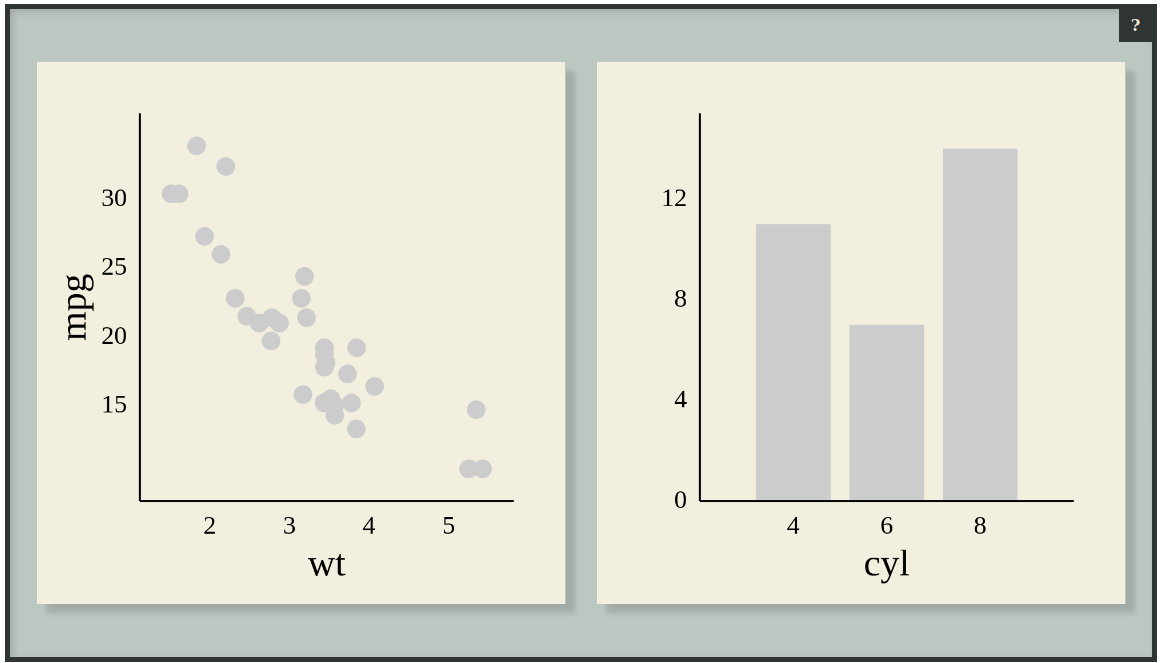
\includegraphics[height=70mm]{./fig_plotscape1.png}
\caption{Creating a basic interactive figure in \texttt{plotscaper} (using \texttt{mtcars} data)}
\label{fig:plotscaperbasic}
\end{figure}

Each Plot consists of one ore more \textbf{Wrangler}(s) and \textbf{Representation}(s). Wranglers take the raw data (shared among all Plots in a Scene) and aggregate them into summary statistics. Representations take these statistics and draw them using graphical primitives, as well as refer back to them during interaction, for example during brushing. Importantly, information from one Wrangler could be used by different representations (e.g. aggegated counts across x- and y- variable could be represented with circles in a bubble plot or squares in fluctuation diagram) and the same Representations can be used to display information from different Wranglers (e.g. barplot and histogram both use bars to display differently derived summary statistics). Wranglers and Representations were implemented in the JavaScript framework of the prototype but were not ported over to the R interface. Finally, each plot also includes a set of \textbf{Scales} and \textbf{Auxilary} graphical objects, such as axis ticks and lines.      

All plots are linked by default, meaning that clicking or clicking-and-dragging over any object will notify the \textbf{Marker} with the corresponding datapoints/cases. The Marker is a global datastructure that is reponsible for imbuing cases in the data with a special status, which changes how the graphical objects that depend on these cases are drawn. For example, as shown in Figure \ref{fig:plotscapertransient}, by default, brushing imbues cases with transient selection, meaning that object/parts of objects that correspond to the selected cases are highlighted, and clicking anywhere else in the figure clears the selection:

\begin{figure}[H]
\centering
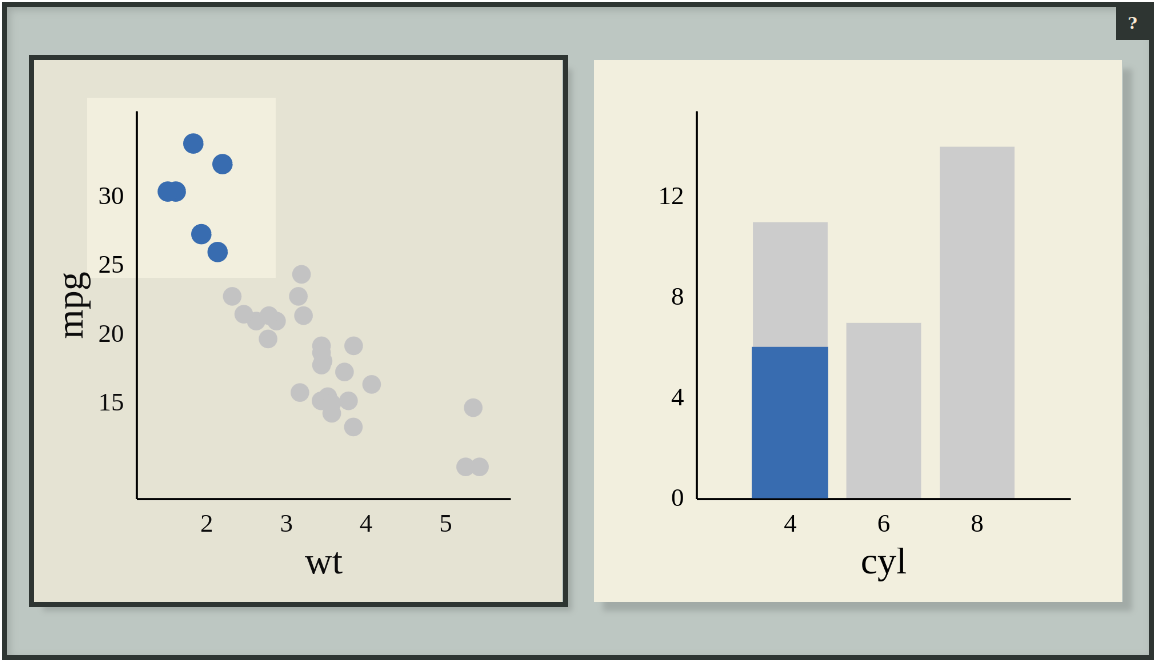
\includegraphics[height=70mm]{./fig_plotscape2.png}
\caption{Transient selection in \texttt{plotscaper}}
\label{fig:plotscapertransient}
\end{figure}

Besides transient selection, the users can also apply persisent selection, by holding down \texttt{1}, \texttt{2}, or \texttt{3} keys while clicking/clicking-and-dragging. This assigns the selected cases to permanent groups shown in different colors, and this selection is not cleared unless the user double-clicks the figure. The user can still apply transient selection, and this will show as a semi-transparent overlay, as long as any permanent selection is present. For example, Figure \ref{fig:plotscaperpersistent} was created by first assinging cases to groups by clicking the bars while holding down the \texttt{1}, \texttt{2}, and \texttt{3} keys, and then brushing an area in the centre of the scatterplot:  

\begin{figure}[H]
\centering
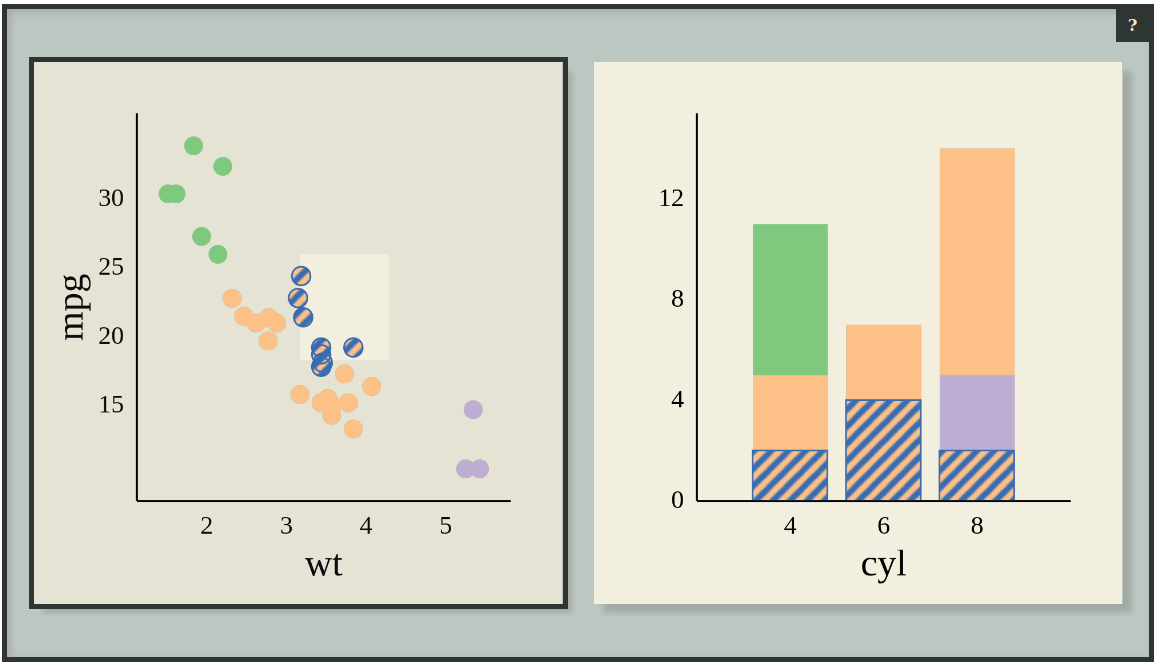
\includegraphics[height=70mm]{./fig_plotscape3.png}
\caption{Combined transient and persisent selection}
\label{fig:plotscaperpersistent}
\end{figure}

The user interaction is managed through \textbf{Handlers}, of which some are global (bound to the Scene) and some local (bound to individual plots). Examples of global handlers includes keyboard handler for keyboard input and state handler for managing which plots are currently active. An example of a local handler is a handler for mouse position/clicking/dragging.  

Besides the global state and Marker, individual Plots have their own state too, which allows for e.g. changing the size/alpha of objects. Besides brushing, panning was also implemented. The implemented types of plots included scatterplot, barplot, histogram, bubbleplot, and fluctuation diagram. Finally, multiple plots could also be arranged into interesting figures using the CSS grid layout, as shown in Figure \ref{fig:plotscaperiris}:

\begin{verbatim}

# Code to create Figure 4

layout <- matrix(c(
  1, 2, 3, 8, 8,
  4, 5, 6, 9, 9,
  7, 7, 7, 10, 10,
  7, 7, 7, 11, 11), ncol = 5, byrow = TRUE)

scene <- ps_scene(iris, layout = layout)

vars <- names(iris)
xyvars <- matrix(vars[combn(1:4, 2)], ncol = 2, byrow = TRUE)

# Add scatterplots
for (i in seq_along(xyvars[, 1])) {
  scene <- scene |> ps_scatter(ps_map(xyvars[i, 1], xyvars[i, 2]))
}

# Add barplot
scene <- scene |> ps_bar(ps_map("Species"))

# Add histograms
for (i in seq_along(names(iris)[-5])) {
  scene <- scene |> ps_histo(ps_map(names(iris)[i]))
}

scene

\end{verbatim}

\begin{figure}[H]
\centering
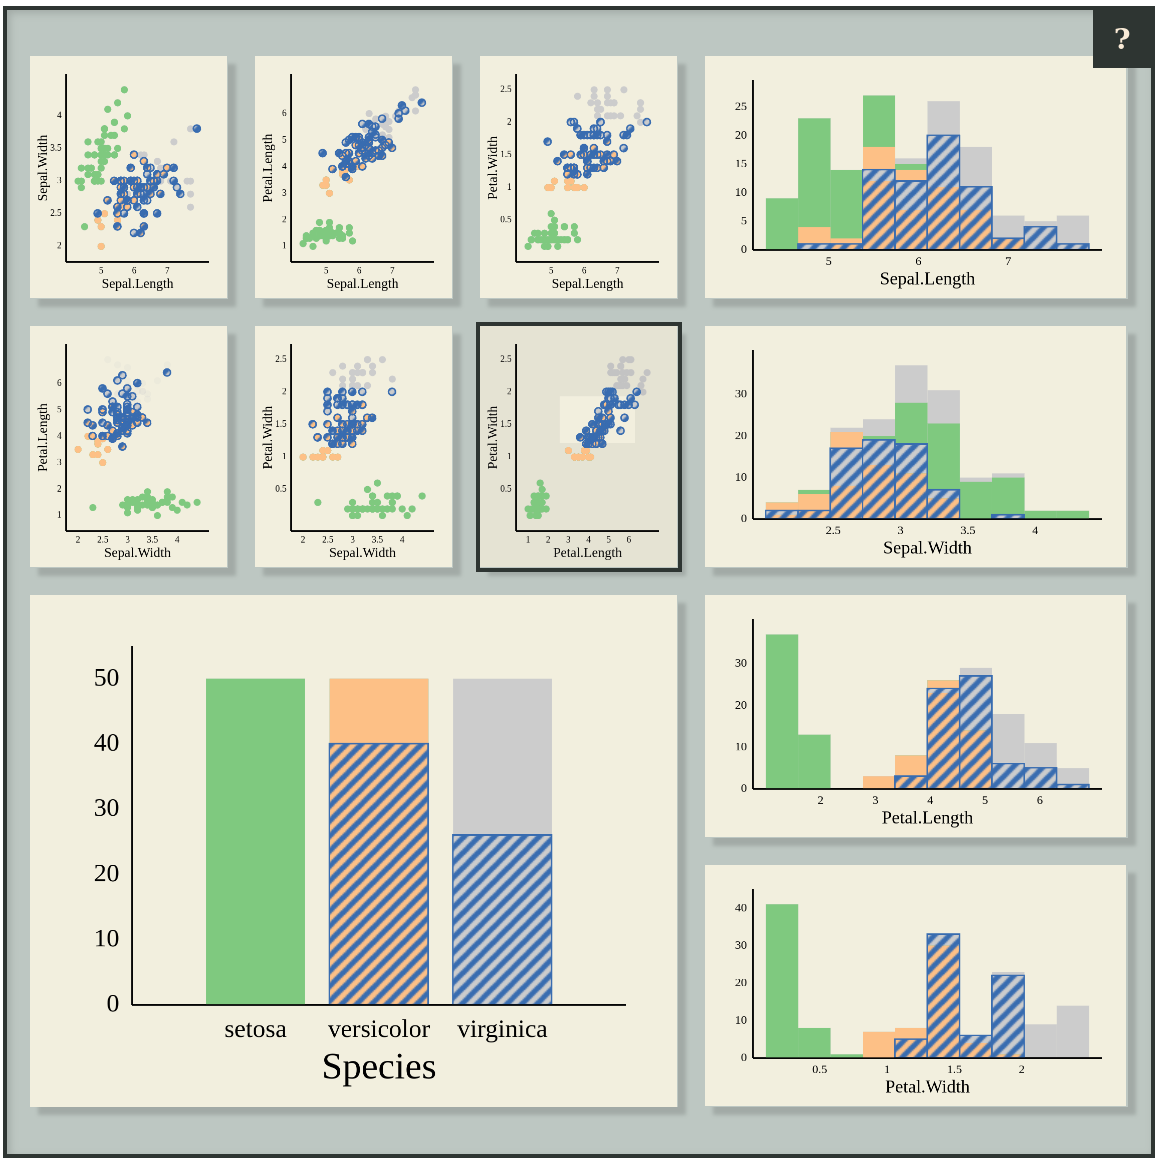
\includegraphics[height=70mm]{./fig_plotscape4.png}
\caption{An interactive figure of the \texttt{iris} dataset}
\label{fig:plotscaperiris}
\end{figure}


\subsection{The Problem of Statistical Summaries}
\label{sec:problem}

Every data visualization has at least one graphical primitive or geometric object that is used to represent some statistical summary of the data. This is true for both static and interactive visualizations. For example, the position of a point on a scatterplot represents the values of the variables on the x- and y-axes. Typically, the statistical summary used in a scatterplot is identity, meaning that the x- and y-position of the point represents the raw values of those variables. As another example, the height of a bar in a histogram conventionally represents the number of cases within a binned range of the x-axis variable. 

In static data visualizations, we are essentially free to compute any kind of statistical summary we like. However, this does not translate to interactive visualizations. Instead, the "interactive" part of interactive data visualization places some contraints on the set of statistical summaries that can be used.  

\subsubsection{Computational Cost and Reactive Cascades}
\label{sec:reactivecascades}

Firstly, there is the problem of computing resources. In static visualizations, we only need to compute each statistical summary once, before we render the plot. However, this may not the case in interactive visualizations. Specifically, if the the summaries can be affected by user input, we can no longer just "fire-and-forget" but instead our system needs to recompute the summaries reactively, whenever interaction happens. For example, if the width of the bins in an interactive histogram changes, we need to recompute the number of cases within each bin. This incurs an additional computational cost. If the statistical summary is too computationally expensive, the volume of data too high, or if the user's input changes too rapidly, it may not be possible to render the graphic smoothly enough. To clarify, this problem only arises when the interaction needs to refer back to the original data (i.e. when the interaction is linked, querying, or parametric, as described in Section \ref{sec:whatcounts}); no extra cost is incurred by e.g. interactively changing the opacity of graphical primitives, irrespective of the data. However, for the more complex and interesting types of interaction, the necessity to recompute summaries reactively can create computational bottlenecks.   

\begin{figure}[H]
\centering
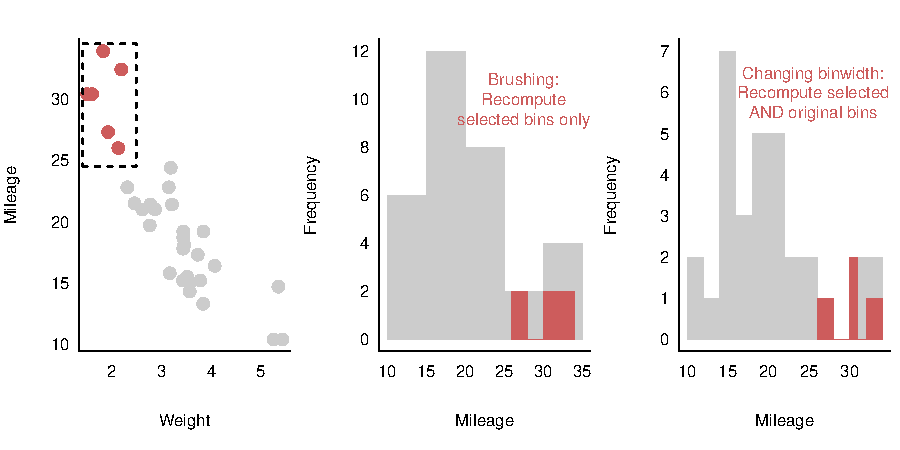
\includegraphics[height=70mm]{./figure03.pdf}
\caption{Reactive computations cascade}
\label{fig:reactivecascade}
\end{figure}

Importantly, these reactive computations can also cascade and form hierarchies. Using the example of the interactive histogram above, if the histogram also responds to linked brushing, reactivity occurs on two different levels, as shown in Figure \ref{fig:reactivecascade}. Firstly, when linked brushing occurs, we only need to recompute the number of (selected) cases within each bin. However, if the width of the bins changes, we need to recompute the histogram breaks \textit{and} the number of cases within each bin (since the bin limits have changed). As such, we can think of the reactive values that underlie the interactive plots as a directed acyclic graph (DAG) - see Figure \ref{fig:dag}. When a value of a node in the DAG changes in response to user input, only the nodes directly downstream of that node should update (but no others). It would be wasteful to e.g. recompute the histogram breaks after brushing. This kind of hierarchy-conscious computation is typical problem that appears in reactive programming \citep[see e.g.][]{doglio2016}, and as such, an efficient implementation of a mid-level interactive data visualization system should be reactive.            

\begin{figure}[H]
\centering
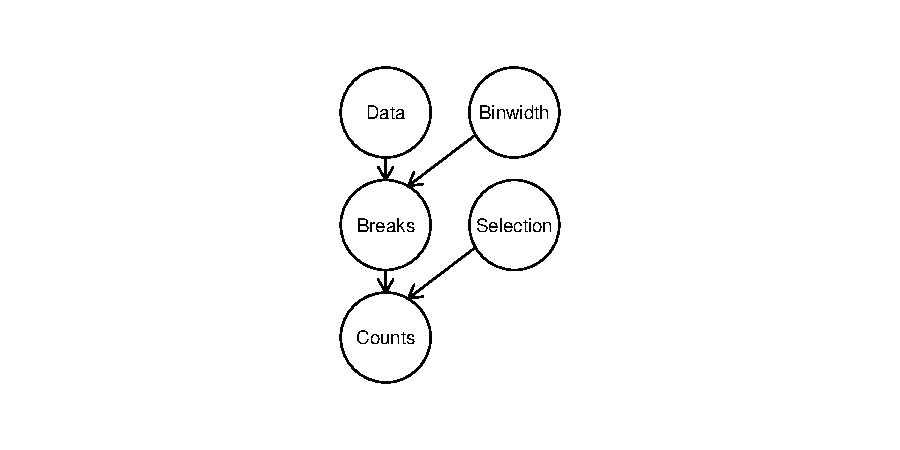
\includegraphics[height=70mm]{./figure04.pdf}
\caption{DAG of a reactive cascade in an interactive histogram}
\label{fig:dag}
\end{figure}

\subsubsection{Visual and Computational Coherency}
\label{sec:coherency}

Perhaps more importantly, different types of interaction also place a limit on what summaries will be computationally and visually coherent. For example, suppose we have a linked barplot and a scatterplot. Further, let's suppose that the barplot displays the means of some other continuous variable (for every level of the x-axis variable). We want the plots to support two-way linked brushing: if the user clicks-and-dragging to select points on the scatterplot, it should highlight parts of the corresponding bars, and vice versa, selecting a bar should highlight the corresponding points.

\begin{figure}[H]
\centering
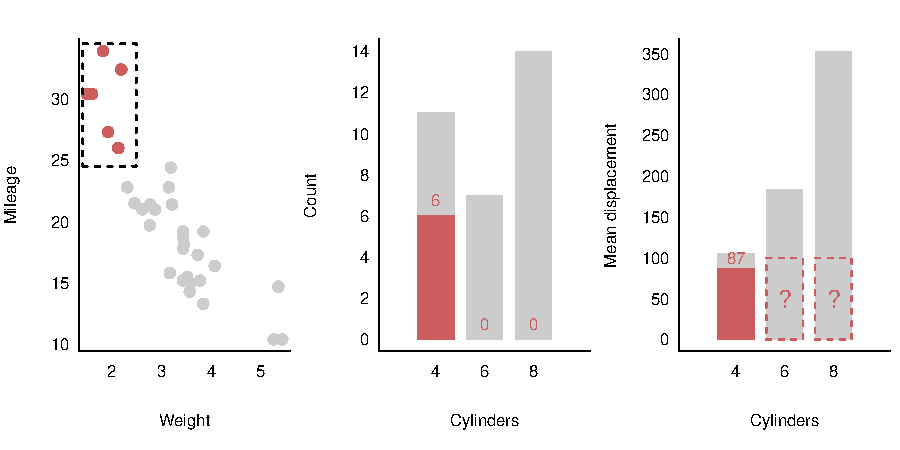
\includegraphics[height=70mm]{./figure01.pdf}
\caption{Sum/count of empty selection is zero but the mean of an empty selection is undefined}
\label{fig:empty}
\end{figure}

We immediately run into several problems. The first is shown in Figure \ref{fig:empty}: how do we draw an empty selection? In a barplot of sums or counts, 0 is a meaningful default value as the sum or count of a set with no elements. However, the mean of an empty set is not defined. We could choose to just not draw the bar of the mean of 0 cases, but this will decouple the statistical summary from the visual representation: now, then the absence of a bar may signal that either no cases are selected or that there are selected cases and their mean is equal to the lower y-axis limit. Conversely, in the barplot of sums, the absence of a bar always indicates that the sum is 0, regardless of whether no cases are selected or whether they all have the value 0 - the visual representation of the statistic is valid either way.  

Second, how do we draw multiple selections? In a sum or count bar, we can stack selected groups on top of each other, and the total height of the stacked bar is always equal to the sum of the heights of the sub-bars, as can be seen in Figure \ref{fig:stacking}. This is not the case for mean: the mean of the group means does not equal the grand mean (except by luck), and there is no other obvious way of combining multiple means. We could draw the group means side-by-side as separate bars (a technique called "dodging" in \texttt{ggplot2}), however, this muddles the two-way reciprocal nature of the linked brushing. Before, the user could simply select the stacked bar as a single, unambiguous entity, they now have to learn by experience whether the dodged group bars can be selected individually or jointly.

\begin{figure}[H]
\centering
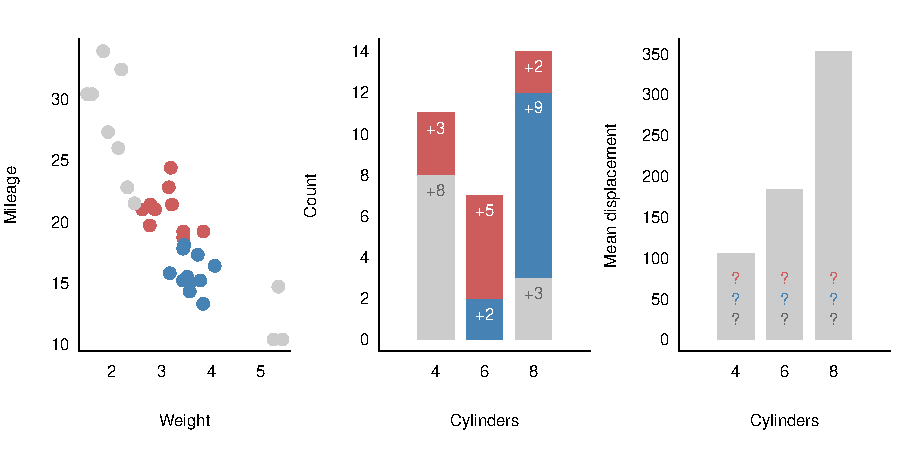
\includegraphics[height=70mm]{./figure02.pdf}
\caption{Sums/counts can be stacked but means cannot}
\label{fig:stacking}
\end{figure}

\subsubsection{Need for Structure}

The picture that emerges is that, when it comes to interactive data visualization, some types of statistical summaries are better than others. Specifically, when more complex types of interactions are desired, such as reciprocal two-way linked brushing, not every kind of statistical summary will do. Some such as count and sum are well-behaved and allow us to represent empty selections and combinations of selections in some obvious or natural way. In other summaries, such as mean, the lack of a sensible default value and the fact that the whole may be different from the sum of its parts leads to a decoupling of the interaction, visual representation, and the statistical summary. It is important to map out the properties that make some summaries "work" and others not. Only by imposing some kind of structure can we lay the foundations for a true mid-level interactive data visualization system. 


\subsection{Few Relevant Bits of (Applied) Category Theory}
\label{ref:categorytheory}

Category theory is a branch of mathematics concerned with the study of universal structures and relations. It was developed as a way of unifying historically distinct areas of mathematics such as abstract algebra, topology, and linear algebra. At the present time, it is also gaining traction in more applied fields, especially computer science and functional programming. Even a very basic complete treatment would be far outside the scope of the present proposal, however, few relevant pieces will be presented in a greatly simplified way, introducing examples from programming when relevant. The treatment here follows mainly from \cite{fong2019} and \cite{Milewski2018}, as well as \cite{leinster2014}.

\subsubsection{Functions}
\label{sec:functions}

Functions are the most fundamental building block of category theory (as well as many other areas of mathematics). In their more general form, they are also known as "morphisms" or "mappings". A function can be described in the following way: given two sets, the set of sources $S$ and the set of targets $T$, a function is a subset $F \subseteq S \times T$ containing all source-target pairs $(s, t)$, such that for all $s \in S$ there exists a unique a $t \in T$. The sets $S$ and $T$ are also known as the domain and codomain, respectively. In programming terms, we should be hypothetically able to implement any function as a lookup table (in practice, this is only feasible when the number of possible arguments is finite and small - but then it can be handy a technique, called \textit{memoization}).  

A function which covers all of its codomain, i.e. one for which, for all $t \in T$, there exists an $s \in S$ such that $f(s) = t$ is called \textit{surjective} or \textit{onto}. A function which has a unique element in the codomain for every element in the domain, i.e. one for which for all $s_1, s_2 \in S$ and $t \in T$, if $f(s_1) = t$ and $f(s_2) = t$, $s_1 = s_2$, is called \textit{injective} or \textit{one-to-one}. Also, for any given subset $T_i \subseteq T$, we can define \textit{pre-image} as the subset of $S$ that maps into $T_i$: $f^{-1}(T_i) = \{ s \in S : f(s) \in T_i \}$. Finally, functions can be composed: if we have two functions $f: X \to Y$ and $g: Y \to Z$, we can combine them into a new function $h = g \circ f$ such that $h: X \to Z$, i.e. $h(x) = g(f(x))$. 

\subsubsection{Partitions}

We can do many things with functions, and one fundamental operation we can do with them is to form \textit{partitions}. Specifically, given a set $A$ and a set of part labels $P$, we can use a surjective function $f: A \to P$ to assign every element in $A$ a part label in $P$. Further, if we then take one of the part labels $p \in P$ and pull it back through $f$ to its pre-image $f^{-1}(p) \subseteq A$, we will then recover the corresponding part $A_p \subseteq A$. We can use this to define partitions in another way, without reference to $f$: a partition of $A$ consists of a set of part labels $P$, such that, for all $p \in P$, there is a non-empty subset $A_p \subseteq A$ and:

$$A = \bigcup_{p \in P} A_p \qquad \text{and} \qquad \text{if } p \neq q, A_p \cap A_q = \varnothing \qquad (\forall p, q \in P)$$

I.e. the parts jointly cover the entirety of $A$ and there is no overlap between their elements. Further, if we have two sets of part labels $P$ and $P'$, and if for every $p \in P$ there exists a $p' \in P'$ such that $A_p = A_{p'}$, the partitions are in some way fundamentally the same. The labels $p \in P$ and $p' \in P'$ may be superficially different, but the two structures encode the same information. This phenomenon is known as \textit{isomorphism}, and will be expounded on in more detail in Section \ref{sec:categories}.  

\subsubsection{Preorders}

Another class of fundamental structures in category theory are preordered sets or \textit{preorders}. A preorder consists of a set $X$ and a binary relation on $X$, often denoted $\leq$, such that:

\begin{enumerate}
\item $x \leq x$ (reflexivity)
\item if $x \leq y$ and $y \leq z$ then $x \leq z$ (transitivity)
\end{enumerate}

Further, if we have one additional property:

\begin{enumerate}
\setcounter{enumi}{2}
\item If $x \leq y$ and $y \leq x$, then $x = y$ (anti-symmetry)
\end{enumerate}

Then we can speak of a partially ordered set, or \textit{poset}. Finally, with one more property:

\begin{enumerate}
\setcounter{enumi}{3}
\item Either $x \leq y$ or $y \leq x$ (comparability)
\end{enumerate}

We can speak of a \textit{total order}. Examples of total orders (which are also by definition posets and preorders) include the set of natural numbers $\mathbb{N}$, reals $\mathbb{R}$, booleans $\mathbb{B} = \{ \text{True, False} \}$, etc... An example of a poset which is not a total order is the tree of life: a species \textit{Homo sapiens} can be thought of as being in a subordinate relationship ($\leq$) to the genus \textit{Homo} and the great ape family, but in no order relationship to another (different) species, e.g. \textit{Canis familiaris}.

\subsubsection{Monoids}

\textit{Monoids} are a simple yet surprisingly useful structure in category theory. Specifically, a monoid is a tuple $(M, e, \otimes)$ consisting of:

\begin{enumerate}
\item An object (set) $M$
\item A "neutral" or "empty" element $e \in M$ called the \textit{monoidal unit}
\item A binary function $\otimes: M \times M \to M$ called the \textit{monoidal product}
\end{enumerate}

Such that, for all $m, m_1, m_2, m_3 \in M$: 

\begin{enumerate}
\renewcommand{\theenumi}{\alph{enumi}}
\item $e \otimes m = m \otimes e = m$ (unitality)
\item $(m_1 \otimes m_2) \otimes m_3 = m_1 \otimes (m_2 \otimes m_3) = m_1 \otimes m_2 \otimes m_3$ (associativity)
\end{enumerate}

In plain English, monoids encapsulate the idea that \textit{the whole is exactly the sum of its parts} (where "sum" can be replaced by any valid monoidal product). Examples of monoids include addition of natural numbers $(\mathbb{N}, 0, +)$, multiplication of reals $(\mathbb{R}, 1, *)$, and matrix multiplication $(\mathbf{Matrix}, \mathbf{I}, \cdot)$, where $\mathbf{I}$ is the identity matrix and the $\cdot$ infix operator is typically omitted by convention. As counterexample, exponentiation is not a monoid, because because it is not associative ($x^{(y^z)} \neq (x^y)^z$). 

Another important aside is that monoids do not need to concern just numerical quantities but the definition is much broader. For example, given any set $S$, the set union $(S, \varnothing, \cup)$ and set intersection $(S, S, \cap)$ are also monoids. String concatenation (e.g. the \texttt{paste()} function in R) is also a perfectly valid monoid: 

\begin{itemize}
\item \texttt{paste("hello", "") == paste("", "hello") == "hello"}
\item \texttt{paste("hello", paste("world", "bye")) == paste(paste("hello", "world"), "bye")}
\end{itemize}

Monoids can be further specialized by imposing additional properties. For example, with:

\begin{enumerate}
\renewcommand{\theenumi}{\alph{enumi}}
\setcounter{enumi}{2}
\item $x \otimes y = y \otimes x$ (commutativity/symmetry)
\end{enumerate}

We can make it so that the direction of applying the monoidal product does not matter (which would still admit regular addition, multiplication, set union, and set intersection, but not matrix multiplication and string concatenation). Additionally, if $M$ is a preorder, we can impose an additional constraint:

\begin{enumerate}
\renewcommand{\theenumi}{\alph{enumi}}
\setcounter{enumi}{3}
\item If $x_1 \leq x_2$ and $y_1 \leq y_2$, $x_1 \otimes y_1 \leq x_2 \otimes y_2$ (monotonicity)
\end{enumerate}

If all four properties a), b), c), and d) hold, we speak of a \textit{symmetric monoidal preorder}. 

In programming, monoids are most typically encountered in the context of arrays, whereby the elements of an array can be iteratively absorbed into a single value, through functions/methods called conventionally \texttt{reduce}, \texttt{fold}, or \texttt{accumulate}. Examples include the \texttt{Reduce()} function in R, the \texttt{fold} function in Haskell, and the \texttt{Array.reduce()} method in JavaScript. As a more concrete example, in JavaScript, \texttt{[1, 2, 3, 4].reduce((x, y) => x + y, 0)} will yield \texttt{10}, \texttt{[1, 2, 3, 4].reduce((x, y) => x * y, 1)} will yield \texttt{24}, and \texttt{["a", "b", "c", "d"].map((x, y) => `\$\{x\}\$\{y\}`, "")} will yield \texttt{abcd}. Importantly, while \texttt{reduce/fold} are most often used with arrays, their generic forms are polymorphic and can be applied to arbitrary datastructures that implement the interface e.g. trees \citep{braithwaite2019}. Finally, one handy, "free" fact about monoids is that they can be readily parallelized: since the end-result of applying the operation recursively to parts is the same as applying it once to the whole, we are free to split and process the data across multiple clusters or machines.  

\subsubsection{Categories}
\label{sec:categories}

The structures we have discussed so far are actually special cases of a much more general concept called \textit{category}. A category $\mathcal{C}$ consists of:

\begin{enumerate}
\item A collection of elements $\text{Ob}(\mathcal{C})$ called the \textit{objects} of $\mathcal{C}$
\item For every pair of objects $a, b \in \text{Ob}(\mathcal{C})$, a set $\mathcal{C}(a, b)$ of \textit{morphisms} from $a$ to $b$ ($f \in \mathcal{C}(a, b)$ can also be denoted $f: a \to b$)
\item For every object $a$, one morphism $\text{id}_a : a \to a$ called the \textit{identity morphism}
\item For every three objects $a, b, c$ and every two morphisms $f : a \to b$ and $g : b \to c$, a \textit{composite morphism} $h : a \to c = g \circ f $ 
\end{enumerate}

Such that:

\begin{enumerate}
\renewcommand{\theenumi}{\alph{enumi}}
\item For any morphism $f: a \to b$, $f \circ id_a = f = id_b \circ f$ (unitality)
\item For any four objects $a_1, a_2, a_3, a_4 \in \text{Ob}(\mathcal{C})$ and morphisms $f: a_1 \to a_2$, $g: a_2 \to a_3$, and $h: a_3 \to a_4$, $h \circ (g \circ f) = (g \circ h) \circ f = g \circ h \circ f$ (associativity)
\end{enumerate}


As was mentioned in Section \ref{sec:functions}, morphisms can be thought of as generalizations of functions: they take one object within a category to another object within the same category, and their composition is associative, just like with regular functions. However, unlike in regular functions, the objects in the category are left unspecified and do not have form a set. The identity morphism guarantees there is always at least one way to start and arrive at the same object, and its composition with other morphisms has no effect.

Preorders can be understood as categories with at most one morphism between any two objects: a morphism $\leq : a \to b$ exists between $a$ and $b$ if and only if $a \leq b$. Transitivity then carries over as composition: if $f: a \to b$ is the relation $a \leq b$, and $g: b \to c$ is the relation $b \leq c$, then $g \circ f$ is the relation $a \leq c$. Similarly, monoids, can be understood as categories with a single (non-identity) morphism, going from itself back to itself. For example, given the monoid $(\mathbb{N}, 0, +)$, we can represent this as a category with a single object $z$ and a morphism $f$ (and identity morphism $id_a$). The identity morphism will then play the role of the monoidal unit $e = id_a$, function composition will play the role of the monoidal product, and the number of times we compose the function will determine the element of the underlying set/preorder: $\{0, 1, 2, \ldots \} = \{id_a, f, (f \circ f), (f \circ f \circ f), \ldots \}$. The associativity and unitality properties of monoids will be fulfilled as a result of the same properties being defined on categories.  

% \subsection{Functors}
% 
% Since morphisms take one object to another within the same category, one can wonder if there is also a way to take one category to another. This leads to the definition of \textit{functors}. To specify a functor $F$ from category $\mathcal{C}$ to category $\mathcal{D}$, denoted as $F: \mathcal{C} \to \mathcal{D}$ we need:
% 
% \begin{enumerate}
% \item For every object $c \in \text{Ob}(\mathcal{C})$, an object $F(c) \in \text{Ob}(\mathcal{D})$
% \item For every morphism $f: a_1 \to a_2$ in $\mathcal{C}$, a morphism $F(f): F(a_1) \to F(a_2)$ in $\mathcal{D}$ 
% \end{enumerate}
% 
% Such that:
% 
% \begin{enumerate}
% \renewcommand{\theenumi}{\alph{enumi}}
% \item For every object $a \in \text{Ob}(\mathcal{C})$, $F(id_a) = id_{F(a)}$
% \item For every three objects $a_1, a_2, a_3 \in \text{Ob}(\mathcal{C})$ and two morphisms $f \in \mathcal{C}(a_1, a_2)$ and $g \in \mathcal{C}(a_2, a_3)$, $F(g \circ f) = F(g) \circ F(f)$
% \end{enumerate}
% 
% This means that, using a functor, we can map objects from one category to another while preserving structure (identity and composition). The mapping does not have to be one-to-one: multiple objects or morphisms in $\mathcal{C}$ can be compressed into a single object/morphism in $\mathcal{D}$. However, the converse is not true: a single object/morphism cannot be split apart into multiple since this would break the identity and composition rules. 
% 
% To give an example of a simple functor, as was mentioned in Section \ref{sec:categories}, pre-orders are categories, and if we take $\mathcal{C}$ to be the preorder on natural numbers $(\mathbb{N}, \leq)$ and $\mathcal{D}$ to be the preorder on booleans $(\mathbb{B}, \leq)$, we can define a functor $F: \mathcal{C} \to \mathcal{D}$ that takes every natural number and maps it to \textbf{False} if it is less than or equal to 5 and to \textbf{True} if it is greater than 5. This preserves identity since e.g. $F(id_4) = id_{\text{False}}$ and also composition, since, remembering that morphisms in pre-orders are order relations, $F(4 \leq 6) = \text{False} \leq \text{True}$ (where $f: 4 \leq 5$, $g: 5 \leq 6$, $g \circ f = 4 \leq 6$, $F(f) = \text{False} \leq \text{False}$, and $F(g) = \text{False} \leq \text{True}$). Functors between pre-orders such as this one are also called \textit{monotone maps}.
% 
% Functors are also a very useful idea in programming since they allow us to abstract away implementation while preserving some kind of behavior (structure). They are typically encountered as endofunctors, i.e. functors that map from a category back to itself. For example, arrays are probably the most popular type of endofunctor and the behavior that they preserve is that functions get applied to every element: e.g. in JavaScript, \texttt{Array.map(f)} will apply \texttt{f} to every element, such that \texttt{[1, 2, 3].map(double) >> [2, 4, 6]}. However, functors can be constructed to preserve any kind of behavior. For example, we could construct a new functor in JavaScript (using OOP Class methods to implement polymorphism) as follows:      
% 
% \begin{verbatim}
% 
% class Timer {
%   
%   constructor(value, times) {
%     this.value = value
%     this.times = times
%   }
%   
%   map = (fun) => {
%     const {value, times} = this
%     const start = performance.now()
%     const result = fun(value)
%     const end = performance.now()
%     times.push(end - start)
%     
%     return new Timer(result, times)
%     }
%     
% }
% 
% \end{verbatim}
% 
% Now, whenever we use a function on an instance of the timer using the \texttt{.map} method, we will simultaneously apply the function and also time its execution and record, e.g. \texttt{new Timer(largeArray, []).map(double).map(square).times} will return an array with two values, one for the time it took to double all values and another for how long it took to square them (after the doubling). It is easy to show that this preserves composition: \texttt{timer.map(double).map(square)} should yield the same result as \texttt{timer.map((x) => square(double(x))} (baring differences in which may arise due to low-level implementation; however, \texttt{timer.value} will be the same).  

This concludes the brief tour of category theory. The treatment above barely scratched the surface, however, it does include some useful ideas in relation to the problems with interactive data visualization systems mentioned in Section \ref{sec:problem}. Specifically, the concepts of partition, monoid, and functor may come handy when reasoning about interactive summaries of the data.  

% ----------------------------------------------------------------------
\section{So What's New?}
\label{sec:whatsnew}

As was laid out in the previous sections, when compared to traditional, static visualization, interactive data visualization presents an idiosyncratic set of challenges and considerations. Specifically, when drawing and interacting with statistical summaries of the data, the user needs to carefully navigate the landscape of these summaries, with only some producing visually and computationally coherent results. The goal of this project is to map out this landscape, and develop theory that will allow everyone to produce coherent interactive graphics. To this end, ideas and concepts from category theory will be used. 

Here's a rough sketch of the model so far:

\begin{itemize}

\item \textbf{Each graphical object represents a partition of the data space.}
  \begin{itemize}
  \item Assuming long data format, each object represents subset of the rows (cases).
  \item One object can represent multiple cases but each case belongs to one object only.
  \item The \textit{entire data space} is also a valid partition: e.g. a time-series line or a density polygon may represent all cases in the data.
  \end{itemize}
  
\item \textbf{The partitions can be nested or sub-partitioned into finer partitions}
  \begin{itemize}

  \item This is most relevant in the case of linked brushing: by interaction (e.g. clicking-and-dragging) we can select object and assign its respective cases to a group.
  \item Each case can belong to one object and one group only; objects can combine multiple groups
  \end{itemize}

\item \textbf{There is a common set of one or more functions (statistical summaries) applied to every partition}

  \begin{itemize}
  \item The outputs of these functions will be used as relevant attributes/dimensions of the graphical objects, e.g. height of bars, area of squares/circles, etc...
  \item The summaries have to be computed on all parts and across all levels of nesting: e.g. if we are counting the number of cases \textit{within each group within each bar}, we also have to count the number of cases \textit{within each bar} (ignoring group), and the number of cases in the data as a whole (ignoring bar and group). 
  \item Forcing the summaries to apply across all partitions consistently will allow for switching between different types of visualizations that represent the same information at different levels of nesting: for example, histograms (count within group within bar for y-coordinate) and spineplots (count within group within bar for y-coordinates \textit{and} count within bar for x-coordinate)
  \end{itemize}

\item \textbf{For coherent two-way interaction, the summaries should form a \textit{symmetric monoidal structure on a total order}}.

  \begin{itemize}
  
  \item I.e. we need a default value for empty selection and a way of combining values, such that the summary on the entire data space is the same as the combined summary of the summaries on the parts
  \item The monoidal product has to be \textit{symmetric}: it should not matter in what order we combine the selections (there is no order to the groups) 
  \item The monoidal product should also be \textit{monotonic}: the combined result of two values has to be greater than or equal to either of the values alone (this property may not be necessary in every type of plot but seems desirable in most).
  \item \textit{Total order} order is required because data visualization is about comparison: every two objects have to be comparable along the relevant dimension. Most often, the total order will be $\mathbb{R}^+$, since so are height, width, area, angle,... 
  \end{itemize}
  
\item \textbf{The computation of the summary function(s) should happen reactively}
  \begin{itemize}
  \item That is, if one level of partitioning changes, only the summary statistics on its children should change but the summary statistics upstream should not be recomputed
  \item For example, in an interactive histogram, linked brushing should not affect breaks, only counts, but changing binwidth should affect both the breaks and counts (see Section \ref{sec:reactivecascades})
  \item An object/class which manages the reactive summaries should hide the reactive implementation from the users
  \end{itemize}

\end{itemize}



The project also seeks to apply the theory above and implement an interactive data visualization system. To this end, a prototype has already been developed in JavaScript and R (available at: \texttt{https://github.com/bartonicek/plotscaper}). Going forward, the following broad goals will be pursued (see Section \ref{sec:goals} for a detailed breakdown):  

\begin{enumerate}

\item Map out the boundaries and constraints of statistical summaries as they relate to interactive data visualization systems 
\item Develop theory for an implementation of a mid-level system
\item Implement the system
\item Communicate the findings

\end{enumerate}


% ----------------------------------------------------------------------
\section{Data and Special Needs}
\label{sec:data}

The use of the system will be tested out on datasets available in the public domain such as the \texttt{diamonds} dataset in R. For these data sets, no ethics or disclosure statements are necessary. Possible collaboration with working scientists and corresponding data access may be negotiated at a later date.  

The student's own personal computer should be sufficient to produce the developing and testing the system. Should extra computing resources become necessary, the student should be able to inquire and be granted access to the \textbf{Ihaka server} (\texttt{ihaka.stat.auckland.ac.nz.}) using SSH connection. Other options such as the New Zealand eScience Infrastructure (\textbf{NeSI}) should be available too. 

The packages produced as part of the project will be published for free as open-source software, under the MIT license \citep{mit2023}. No additional ethics approvals are necessary. 

% ----------------------------------------------------------------------
\section{Budget}

Development of open-source software is not very budget-intensive. The work related to the project will be funded by the University of Auckland Doctoral Scholarship. Expenses related to conferences (registration fees, travel) may be funded via the Postgraduate Research Student Support (PReSS) account, with an annual allocation of \$1200 NZD. 

% ----------------------------------------------------------------------
\section{Objectives and Goals}
\label{sec:goals}


The objective(s) of this research project are to:

\begin{enumerate}

\item
Map out boundaries and constraints that statistical summaries in a mid-level interactive data visualization system should meet
  \begin{enumerate}
  \item Describe what contracts do graphical primitives and underlying statistical summaries need to uphold in order to be interactable with in a coherent and predictable way
  \item Use concepts from category theory to describe the necessary structures
  \item Consider links to functional programming  
  \end{enumerate}

\item Implement the system in JavaScript (provisionally named \texttt{plotscape})
  \begin{enumerate}
  \item Use mainly plain ES2020, possibly incorporate basic utility libraries such as a reactive programming library and functional programming library
  \item Use the HTML \texttt{canvas} element as a drawing utility, explore using WebGL and other frameworks for performance
  \item Profile and test relevant parts of the code
  \item Publish as an \texttt{npm} package
  \item Provide a full documentation for any functions, classes, etc...
  \end{enumerate}

\item Implement a high-level interface to the system in R (provisionally named \texttt{plotscaper})
  \begin{enumerate}
  \item Provide a full documentation for all functions
  \item Provide a package vignette
  \item Pass all \texttt{CRAN} checks and publish on \texttt{CRAN} 
  \end{enumerate}
  
\item Publish an article in a peer-reviewed academic journal such as the \textit{Journal of Statistical Software}

\item Present finding at conferences and user groups such as \textbf{useR!} or \textbf{IEEE VIS}

\end{enumerate}

% ----------------------------------------------------------------------
\section{Deliverables and Program Schedule}
\label{sec:timeline}




\begin{table}[hh]
\caption{
Timeline for my thesis.
Itemize the list of deliverables with specific dates so that
you can make concerted effort to achieve them.
Here are \textit{some} activities---fill in more.
}
\centering
\ ~~~~ \\
\label{tab:timeline}
\begin{tabular}{|c|l|}
\hline
Date & Activity \\
\hline
2022-03-01 & Enrolled in Research Master's in Statistics, backdated provisional PhD registration. \\
2022-11-07 & Made a Github commit of the initial fully working prototype of \texttt{plotscaper}. \\
2022-11-22 & Gave talk at the NZSA Unconference, received Outstanding Student Presentation award. \\
2023-02-13 & Completed DELNA. \\
2023-03-10 & Attended central doctoral induction. \\
2023-04-07 & Presented my research at Iowa State University Graphics Group \\
2023-04-13 & Attended FoS doctoral induction. \\
2023-05-14 & Present my research at a PYR seminar \\
2023-08-01 & Finalize version 1.0 of \texttt{plotscape} and publish on \texttt{npm} \\
2023-09-01 & Attend a statistical computing/data visualization conference \\
2023-12-01 & Submit my first paper to \textit{Journal of Statistical Software} (co-authored with supervisors). \\
2024-01-01 & Finalize version 1.0 of \texttt{plotscaper} and publish on \texttt{CRAN}. \\
2024-03-01 & Begin work on formalizing the manuscript \\
2024-06-01 & Attend a statistical computing/data visualization conference \\
2025-03-01 & Submit the thesis. \\
\hline
\end{tabular}
\end{table}



I have fulfulled all my first year requirements. These are:

\begin{enumerate}

\item \textit{Attend the Central Doctoral Induction}: 2023-03-10
\item \textit{Attend the FoS Doctoral Induction}: 2023-04-13
\item \textit{Complete DELNA screening}: 2023-02-13
\item \textit{Complete a health and safety risk assessment (if required)}: not required
\item \textit{Gain ethics approval (if required)}: not required
\item \textit{Complete training and development needs analysis}: completed prior to transferral from Research Master's
\item \textit{Gain approval for your full thesis proposal}: in process
\item \textit{Give an oral presentation of your work}: PYR seminar being scheduled for May
\item \textit{Produce a substantial piece of written work}: roughly 80~percent Research Master's thesis submitted to primary supervisor for review, 
code repositories available for review on Github at \texttt{https://github.com/bartonicek}
\item \textit{Discuss your research with your Confirmation Review Committee}: in process \newline \newline

Additional first year milestones:

\item \textit{Attend 10 departmental seminars}: Currently 9 attended, I have had only about 3 months to attend departmental seminars but have tried to attend as many as possible.
\item \textit{Engage with other scholars}: Presented research at the NZSA Uncoference 2022 (and received an award) as well as at Iowa State University Graphics Group
\item \textit{Review existing methods and literature on approaches to interactive statistical graphics}: Completed as part of the submitted draft of Research Master's Thesis
\item \textit{Implement a software prototype capable of producing linked interactive plots with support for different types of brushing}: implemented in \texttt{plotscape}


\end{enumerate}


\begin{table}[H]
\caption{
\textbf{Seminars I have attended}.
First section includes departmental seminars and talks (talks count as 1/2 of seminar).
Second section includes seminars from another UoA department.
Third row includes conference talks.
Fourth row includes talks I presented (these do not count towards seminar attendance as far as I am aware but I thought it may still be useful to include them) \newline
\textbf{Note}:
I filled in the required document and submitted it within the required time period after each seminar I attended.
}
\centering
\ ~~~~ \\
\label{tab:seminars}
\begin{tabular}{|c|l|p{10cm}|}
\hline
Date & Speaker & Title \\
\hline
2023-01-27 & Bradley Drayton &
A Talk About Simulations \\
%
2023-02-10 & Rob Gould &
K-12 Data Science or Statistics? Is a Distinction Needed? \\
%
2023-02-22 & Maartje van de Vrugt &
Experiences of an OR Specialist Advising in a Hospital: Reducing Cancellations and
Scheduling Re-work at Outpatient Departments of Amsterdam UMC \\
%
2023-03-07 & Chaitanya Joshi &
Eliciting Informative Priors using Expert decision-making \\
%
2023-03-07 & Fabrizio Ruggeri &
Fast and Likelihood-Free Parameter Estimation for Dynamic Queueing Networks: The
Case of the Immigration Queue at an International Airport \textit{(counts as 1/2 seminar)} \\
%
2023-03-07 & Petra Tang &
A Parametric Approach to estimate Spectral Density of Gravitational Wave Signal from
BPASS Galactic White Dwarf Binary Population \textit{(counts as 1/2 seminar)} \\
%
2023-03-30 & Matt Edwards &
The Good, the Bad, and the Ugly of Working at StatsNZ \\
%
2023-04-21 & Godrick Oketch &
Saddlepoint Methods and Estimation: A new
framework \textit{(counts as 1/2 seminar)} \\
%
2023-04-21 & Jesse Goodman & 
Factoring the saddlepoint approximation across
the Markov property for recursively compounded processes \textit{(counts as 1/2 seminar)} \\

\hline

2023-04-12 & Christopher Horvat &
How Do the Floes Flow? Discrete-Element Modelling of Sea Ice-Ocean Dynamic Coupling in the Marginal Ice Zone. \newline Department of Physics. \\

\hline

2022-11-23 & Tilman Davies & Nearest-Neighbour Gaussian Processes. \newline NZSA Unconference 2022. \\

\hline
%
2022-11-22 & Adam Bartonicek (presented) & Interactive Data Exploration with \texttt{plotscaper}. \newline NZSA Unconference 2022 \\
%
2023-04-07 & Adam Bartonicek (presented) & \textit{Same title as above}. \newline Iowa State University Graphics Group \\

\hline

\end{tabular}
\end{table}








% ----------------------------------------------------------------------
\section*{Appendix~A}

\addcontentsline{toc}{section}{References}
\bibliographystyle{./elsart-harv} % elsart-harv,plain,unsrt,alpha
\bibliography{./references}



\end{document}


